%%% additional documentclass options:
%  [doublespacing]
%  [linenumbers]   - put the line numbers on margins

%%% loading packages, author definitions

%\documentclass[twocolumn]{bmcart}% uncomment this for twocolumn layout and comment line below
\documentclass{bmcart}
\usepackage[utf8]{inputenc}
\usepackage{amsmath}
\usepackage{amssymb}
\usepackage{graphicx}
\usepackage[font=scriptsize,labelfont={bf}]{caption}
\usepackage[justification=raggedright,nearskip=10pt,farskip=0pt]{subfig}
\usepackage{calc}
\usepackage{url}
\usepackage{array}
\usepackage{rotating}
\usepackage{tabularx}
\usepackage{multirow}
\usepackage{layouts}
\usepackage{titletoc}
\usepackage{setspace}
\usepackage{longtable}
\usepackage{pgf}
\usepackage{tikz}
\usetikzlibrary{shapes,arrows}
\usepackage{footnote}

%%%%%%%%%%%%%%%%%%%%%%%%%%%%%%%%%%%%%%%%%%%%%%%%%
%%                                             %%
%%  If you wish to display your graphics for   %%
%%  your own use using includegraphic or       %%
%%  includegraphics, then comment out the      %%
%%  following two lines of code.               %%
%%  NB: These line *must* be included when     %%
%%  submitting to BMC.                         %%
%%  All figure files must be submitted as      %%
%%  separate graphics through the BMC          %%
%%  submission process, not included in the    %%
%%  submitted article.                         %%
%%                                             %%
%%%%%%%%%%%%%%%%%%%%%%%%%%%%%%%%%%%%%%%%%%%%%%%%%
% \def\includegraphic[#1]#2{}
% \def\includegraphics[#1]#2{}

%%% Put your definitions there:
\startlocaldefs
\hbadness=9999999 %avoid complaining for underfull h/vbox
\vbadness=9999999

% \setlength{\columnwidth}{86mm}
 \captionsetup[subfloat]{labelformat=empty} %position=top, justification=raggedright, singlelinecheck=false, labelformat=simple, font={scriptsize,sf,bf}, width=0.5\textwidth}
 \captionsetup{width=0.95\textwidth, indention=-12pt}
 \renewcommand*\thesubfigure{\Alph{subfigure}}
 \setlength{\belowcaptionskip}{-3mm}
 %\setlength{\abovecaptionskip}{0mm}
%\addtolength{\abovecaptionskip}{-3mm}

%\subfiguretopcaptrue

\pdfminorversion=4
\pdfobjcompresslevel=0

\pgfdeclareimage[height=3ex]{win-logo}{images/win_logo}
\pgfdeclareimage[height=3ex]{mac-logo}{images/mac_logo}
\pgfdeclareimage[height=3ex]{linux-logo}{images/linux_logo}
\pgfdeclareimage[height=3ex]{ubuntu-logo}{images/ubuntu_logo}
\pgfdeclareimage[height=2ex]{mac-command}{images/mac_command}
\pgfdeclareimage[height=2ex]{lower-bound}{images/lowerbound}
\pgfdeclareimage[height=2ex]{upper-bound}{images/upperbound_green}
\pgfdeclareimage[width=0.95\textwidth]{FigS10}{Figures/S10}
\pgfdeclareimage[width=0.95\textwidth]{FigS11}{Figures/S11}
\pgfdeclareimage[width=0.95\textwidth]{FigS12}{Figures/S12}
\pgfdeclareimage[width=0.95\textwidth]{FigS6}{Figures/S6}

\newcommand{\winsymbol}{\raisebox{-0.8ex}{\pgfuseimage{win-logo}}}
\newcommand{\macsymbol}{\raisebox{-0.5ex}{\pgfuseimage{mac-logo}}}
\newcommand{\linuxsymbol}{\raisebox{-0.8ex}{\pgfuseimage{linux-logo}}}
\newcommand{\ubuntusymbol}{\raisebox{-0.9ex}{\pgfuseimage{ubuntu-logo}}}
\newcommand{\winmaclinux}[3]{\begin{itemize}
    \item[\winsymbol] #1
    \item[\macsymbol] #2
    \item[\linuxsymbol] #3
\end{itemize}}
\newcommand{\macpc}[2]{\begin{itemize}
    \item[\macsymbol] #1
    \item[\winsymbol\ \  \linuxsymbol] #2
\end{itemize}}

\newcommand{\maccmd}{\raisebox{-0.35ex}{\pgfuseimage{mac-command}}}

\setlength{\abovecaptionskip}{1.3mm}
%\setlength{\belowcaptionskip}{1mm}

\def\ta{Timed Automaton}
\def\tas{Timed Automata}
\def\animo2{ANIMO 2}

%\setvaluelist{bmcsymbol}{*,\textdagger,\^{}}
\def\textdagger{\#{}} %I would be very happy to avoid the distasteful symbol \textdagger (or \dagger, whatever).

%\def \doiurl#1{\textsf{#1}}

\endlocaldefs

\makeindex

\begin{document}

\begin{frontmatter}

\begin{fmbox}
\dochead{Methodology}

\title{Modelling with ANIMO:\\ between Fuzzy Logic and Differential Equations}

%%%%%%%%%%%%%%%%%%%%%%%%%%%%%%%%%%%%%%%%%%%%%%
%%                                          %%
%% Enter the authors here                   %%
%%                                          %%
%% Specify information, if available,       %%
%% in the form:                             %%
%%   <key>={<id1>,<id2>}                    %%
%%   <key>=                                 %%
%% Comment or delete the keys which are     %%
%% not used. Repeat \author command as much %%
%% as required.                             %%
%%                                          %%
%%%%%%%%%%%%%%%%%%%%%%%%%%%%%%%%%%%%%%%%%%%%%%

\author[
   addressref={aff1},                   % id's of addresses, e.g. {aff1,aff2}
   %corref={aff1},                       % id of corresponding address, if any
   noteref={n1},                        % id's of article notes, if any
   email={s.schivo@utwente.nl}   % email address
]{\inits{S}\fnm{Stefano}~\snm{Schivo}}
\author[
   addressref={aff2},
   noteref={n1},
   email={j.scholma@utwente.nl}
]{\inits{J}\fnm{Jetse}~\snm{Scholma}}
\author[
   addressref={aff3},
   email={p.e.vandervet@utwente.nl}
]{\inits{PE}\fnm{Paul E.}~\snm{van~der~Vet}}
\author[
   addressref={aff2},
   email={h.b.j.karperien@utwente.nl}
]{\inits{M}\fnm{Marcel}~\snm{Karperien}}
\author[
   addressref={aff2},
   %corref={aff2},
   email={j.n.post@utwente.nl}
]{\inits{JN}\fnm{Janine N.}~\snm{Post}}
\author[
   addressref={aff1},
   %corref={aff1},
   email={j.c.vandepol@utwente.nl}
]{\inits{J}\fnm{Jaco}~\snm{van~de~Pol}}
\author[
   addressref={aff1},
   corref={aff1},
   email={r.langerak@utwente.nl}
]{\inits{R}\fnm{Rom}~\snm{Langerak}}

%%%%%%%%%%%%%%%%%%%%%%%%%%%%%%%%%%%%%%%%%%%%%%
%%                                          %%
%% Enter the authors' addresses here        %%
%%                                          %%
%% Repeat \address commands as much as      %%
%% required.                                %%
%%                                          %%
%%%%%%%%%%%%%%%%%%%%%%%%%%%%%%%%%%%%%%%%%%%%%%

\address[id=aff1]{%                           % unique id
  \orgname{Formal Methods and Tools, Faculty of EEMCS, University of Twente}, % university, etc
  \street{P.O. Box 217},                     %
  \postcode{7500AE}                           % post or zip code
  \city{Enschede},                              % city
  \cny{The~Netherlands}                                    % country
}
\address[id=aff2]{%
  \orgname{Developmental BioEngineering, MIRA Institute for Biomedical Technology and Technical Medicine, University of Twente},
  \street{P.O. Box 217},                     %
  \postcode{7500AE}                           % post or zip code
  \city{Enschede},
  \cny{The~Netherlands}
}
\address[id=aff3]{%
  \orgname{Human Media Interaction, Faculty of EEMCS, University of Twente},
  \street{P.O. Box 217},                     %
  \postcode{7500AE}                           % post or zip code
  \city{Enschede},
  \cny{The~Netherlands}
}

%%%%%%%%%%%%%%%%%%%%%%%%%%%%%%%%%%%%%%%%%%%%%%
%%                                          %%
%% Enter short notes here                   %%
%%                                          %%
%% Short notes will be after addresses      %%
%% on first page.                           %%
%%                                          %%
%%%%%%%%%%%%%%%%%%%%%%%%%%%%%%%%%%%%%%%%%%%%%%

\begin{artnotes}
%\note{Sample of title note}     % note to the article
\note[id=n1]{Equal contributor} % note, connected to author
\end{artnotes}


\end{fmbox}% comment this for two column layout


\maketitle

%%%%%%%%%%%%%%%%%%%%%%%%%%%%%%%%%%%%%%%%%%%%%%
%%                                          %%
%% The Abstract begins here                 %%
%%                                          %%
%% Please refer to the Instructions for     %%
%% authors on http://www.biomedcentral.com  %%
%% and include the section headings         %%
%% accordingly for your article type.       %%
%%                                          %%
%%%%%%%%%%%%%%%%%%%%%%%%%%%%%%%%%%%%%%%%%%%%%%

\begin{abstractbox}

\begin{abstract} % abstract <= 350 words. Headers: background, results, conclusions
\parttitle{Background}
Experimental biologists need to deal with large amounts of data on a daily basis.
This makes computational support essential in order
to reason on the dynamics of biological systems.
The software tool ANIMO (Analysis of Networks with Interactive MOdelling)
provides such computational support and allows insight into the complex networks of signalling events occurring in living cells.
Biology experts are able to exploit the power of the underlying formal methods
via a user interface specifically tailored for biological applications. Knowledge
of the underlying formalisms is not necessary to use ANIMO.
\parttitle{Results}
ANIMO models show a degree of precision intermediate between ordinary differential equations (ODEs) and fuzzy logic.
We show this by presenting ANIMO models for two case studies: \emph{Drosophila melanogaster} circadian clock, and signal
transduction events downstream of TNF$\alpha$ and EGF in HT-29 human
colon carcinoma cells.
The models were originally developed with ODEs and
fuzzy logic, respectively.
\parttitle{Conclusions}
ANIMO models replicate with good precision the results of both the ODE and
fuzzy logic models. Moreover, ANIMO models require less parameters than ODEs and are more precise than
fuzzy logic. For this reason we position the modelling paradigm of ANIMO
between ODEs and fuzzy logic.
\end{abstract}

%%%%%%%%%%%%%%%%%%%%%%%%%%%%%%%%%%%%%%%%%%%%%%
%%                                          %%
%% The keywords begin here                  %%
%%                                          %%
%% Put each keyword in separate \kwd{}.     %%
%%                                          %%
%%%%%%%%%%%%%%%%%%%%%%%%%%%%%%%%%%%%%%%%%%%%%%

\begin{keyword}
\kwd{modelling}
\kwd{signalling pathway}
\kwd{timed automata}
\kwd{dynamic behaviour}
\end{keyword}

% MSC classifications codes, if any
%\begin{keyword}[class=AMS]
%\kwd[Primary ]{}
%\kwd{}
%\kwd[; secondary ]{}
%\end{keyword}

\end{abstractbox}
%
%\end{fmbox}% uncomment this for twcolumn layout

\end{frontmatter}


\section*{Background}\label{sec:introduction}
\subsection*{Modelling in cell biology}
Executable biology is a young subfield in computational modelling, aimed at constructing models that mimic
biological phenomena \emph{in silico}. It provides an interesting paradigm 
to enhance network diagrams with an underlying formal description of network components
and their interactions. Executable models typically contain descriptions of the 
direct interactions of network components, requiring the modeller to think in terms of
``cause and effect''. Biologists reason in similar ways about the molecular mechanisms of network
interactions, and this makes the construction of an executable model an intuitive process.
ANIMO (Analysis of Networks with Interactive MOdelling,~\cite{animo-ieee,animo-gene})
provides an enabling technology to increase the use of computational models by experimental
biologists using their domain-specific language. 
ANIMO enriches the normally static biological network diagrams with dynamic information,
which is then used to automatically produce formal models representing the biological network.
Such models are indispensable for formally
comparing experimental data with prior knowledge, or for structuring experimental findings into a
new theory.
When dealing with complex biological networks, executable biology models are particularly useful
to understand the non-linear dynamics and the entailed emergent properties of the networks.
In those cases, an ANIMO model can be used as a support to obtain insight based on abstract
representations of the interactions occurring inside living cells.
Other applications of ANIMO models include performing \emph{in silico} experiments and
the storage and transfer of knowledge on biological networks.

\subsection*{A brief introduction to ANIMO}
The user interface of ANIMO is displayed in Figure~\ref{fig:cytoscape},
where we present an example of a biological network enriched with dynamic information.
ANIMO is implemented as a plug-in to Cytoscape~\cite{cytoscape}, a software tool developed to represent biological networks.
On top of the static topological information displayed in Cytoscape, ANIMO represents
biological interactions starting from the basic concept of \emph{activity}:
each biological entity in an ANIMO model is considered to be either active or inactive.
Activity is to be interpreted in a very broad sense: for example, an active gene is being transcribed,
an active kinase can perform phosphorylations, etc. Each node in an ANIMO network represents
both active and inactive entities of the same type, with the relative amount of active entities
(the \emph{activity level}) represented by the node colour on a user-configurable scale.
Interactions among nodes define how the biological entities in a network influence each other's activity.
Only nodes whose activity level is larger than 0 (such nodes are called \emph{active}) can have an 
influence on their downstream targets, and only if that influence is not counterbalanced by intervening opposite interactions.
For example, the interaction $A\rightarrow B$ (read ``A activates B'') indicates that node A, if active,
will increase the activity level of node B. If we add an additional interaction to the example,
$C \dashv$\hspace{0.1em}$B$ (``C inhibits B''), with C also active, then the activity level of B will change depending on the
activity levels of A and C, and on their quantitative influence.
The influence of an ANIMO interaction is quantified by a parameter $k$, which defines the speed at which
that interaction occurs: higher values of $k$ give faster interactions. These $k$-values are
the only parameters needed in an ANIMO model, and can be given in either
a quantitative (as real numbers) or a qualitative way, choosing among self-explanatory descriptions
such as ``very slow'', ``slow'', ``medium'', ``fast'', ``very fast''.





ANIMO produces graphs showing how the activity levels of selected nodes
change over time, allowing the user to obtain a view on the dynamic behaviour of their network.
In order to obtain these results, a model defined in ANIMO is automatically translated into
its corresponding representation as a network of Timed Automata~\cite{timed-automata-alur-dill}
and then analysed \emph{behind the scenes} with the software tool UPPAAL~\cite{uppaal}.
The formal language of Timed Automata allows to represent and analyse complex behaviours precisely and efficiently,
but the user does not need to directly manipulate Timed Automata or UPPAAL, as the analysis process is made transparent.
A fastidious user can still access the underlying models and perform other analyses in UPPAAL,
but that is not required in order to fully profit from ANIMO.

A detailed description on how the Timed Automata models defined by ANIMO work, and how the results are obtained,
can be found in~\cite{animo-ieee}. The choice of parameters for ANIMO models is described in~\cite{animo-syncop}.
Additional guidance on the design of ANIMO models and how to best profit from biological experimental data can be found in~\cite{animo-gene}.

Figure~\ref{fig:animo-spectrum} shows the position of ANIMO in a spectrum of modelling methods: justification for this placement is given in the Results section.






\section*{Results}\label{sec:results}
\subsection*{Modelling oscillation in Drosophila Melanogaster circadian clock}\label{sec:animo-drosophila}
To demonstrate that results obtained with ANIMO are comparable to results from widely used modelling
approaches, we present 
an ANIMO model of the circadian clock in \emph{Drosophila Melanogaster} (Suppl. Fig.~S4). %\ref{fig:drosophila-model}).
This ANIMO model is based on~\cite{drosophila-ode-model},
where ordinary differential equations (ODEs) were used.
The cyclic behaviour of the circadian clock is based on the alternating formation and destruction of the
CYC/CLK protein complex.
Concentration levels of this complex are in turn regulated by a series of proteins which are produced as
a consequence of CYC/CLK formation. The CWO protein
is central to the functioning of the network, as it degrades the mRNA for most of the involved proteins.
As such, CWO acts as an inhibitor that counterbalances the effect of CYC/CLK.
The positive influence of the light-regulated cryptochrome CRY on the degradation of TIM is a consequence
of the passage between day and night, allowing
the circadian clock to synchronize to a time zone (see Suppl. Sect.~D.2). %\ref{suppl:repressilator}).


The output of the ANIMO model (see Suppl. Fig.S4) %~\ref{fig:drosophila-model})
matches the original ODE model.
In particular, the oscillations in both models show similar periods and phases (see Fig.~\ref{fig:grafici-drosophila-smaller} for
an example, and Suppl. Fig~S6 %\ref{suppl-fig:grafici-drosophila}
for the complete comparison).
Details of the comparison
between the ANIMO model and the original ODE model are given in Supplementary Section D.3. %~\ref{suppl-sec:animo-drosophila}.








\subsection*{Using ANIMO to generate hypotheses in human colon carcinoma cells}\label{subsec:case-study-larger}
We now present a comparison with an existing fuzzy logic model, which we use also as an example of how
ANIMO can be used to create reference models and help to obtain insight into complex biological events.

We constructed a model of the signalling network downstream of TNF$\alpha$ and EGF
in HT-29 human colon carcinoma cells, formalizing
the crosstalk that takes place between the pathways at different levels of cellular regulation.
We first modelled the two pathways in isolation~(Suppl. Figs.~S7, S8), %\ref{fig:large-model-tnf}, \ref{fig:large-model-egf}),
using information on protein interactions from
the KEGG~\cite{kegg} and phosphosite~\cite{phosphosite} databases. These models were fitted to experimental data
from previous studies~\cite{pathway-compendium,pathway-autocrine}.
We then merged the two pathways into a single model and added autocrine crosstalk between the pathways that has been
described in~\cite{pathway-autocrine}.
Briefly, stimulation with TNF$\alpha$ ({\sf TNFa} in the model) leads to a rapid release of TGF$\alpha$ ({\sf TGFa}),
which activates the EGF receptor ({\sf EGFR}).
This activation causes secretion of IL-1$\alpha$ ({\sf IL-1a}) at later time points.
The effect of IL-1$\alpha$ is down-regulated by the secretion of IL-1 receptor antagonist ({\sf IL-1ra})
downstream of TNF$\alpha$.
The resulting model (Fig.~\ref{fig:large-model-all}A) was compared to the experimental data
for treatments with 100 ng/ml TNF alone and 100 ng/ml EGF alone (data not shown)~\cite{pathway-compendium}.




At this point, the behaviour of the model deviated from the data for some of the nodes.
Changing the parameters of the model was not enough to reproduce the behaviour shown by experimental
data. This is an interesting situation, as it requires changes in the topology of
the model~\cite{animo-syncop}, reflecting the formulation of a new hypothesis
on the structure of the model. Below, we give two examples and show how
adaptation of the model can be used to generate novel testable hypotheses.





Experimentally,
treatment with TGF$\alpha$ alone does not lead to secretion of IL-1$\alpha$. Instead, a co-stimulation with
TGF$\alpha$ and TNF$\alpha$ is required~\cite{pathway-autocrine}.
However, in the first version of the model, treatment with TGF$\alpha$ was sufficient for
IL-1$\alpha$ expression (Fig.~\ref{fig:large-model-all}B). Given the time delay until secretion of IL-1$\alpha$, it can be
expected that \emph{de novo} synthesis of IL-1$\alpha$ is required and that both
TNF$\alpha$ and TGF$\alpha$ are needed to activate transcription of the IL-1$\alpha$ gene.
JNK1 and ERK signal downstream of TNF$\alpha$ and TGF$\alpha$, respectively, and are known
to affect the activity of multiple transcription factors. We altered the model to make
activation of IL-1$\alpha$ expression dependent on both JNK1 activity and ERK activity
(Suppl. Fig.~S9, %\ref{fig:large-model-hypotheses}, 
arrows linking {\sf JNK1} and {\sf ERK} to {\sf IL-1a gene}).
After this modification to the model, IL-1$\alpha$ was no longer secreted
upon stimulation with TGF$\alpha$ alone, which greatly improved the fit between the measured IL-1$\alpha$
levels and the model (Fig.~\ref{fig:large-model-complete}B). This hypothesis could now be used to
design a new experiment to validate IL-1$\alpha$ as a target of combined JNK1 activity and ERK activity in
HT-29 cells. For example, kinase inhibitors specific to JNK1 and ERK could be used to confirm that activity of
both kinases is required for expression and secretion of IL-1$\alpha$. Performing the experiment is beyond
the scope of this study, but this hypothesis finds support in literature:
transcription factors c-Jun and c-Fos together
form a heterodimer known as AP-1 and are activated by JNK1 and ERK,
respectively~\cite{jnk-signaling,cfos-cjun}. AP-1 has been reported to bind to the
promoter of IL-1$\alpha$, providing evidence for a role in the regulation of IL-1$\alpha$
expression~\cite{ap1-il1a}. Based on these findings in literature we included c-Jun and
c-Fos in our model as transcriptional activators of IL-1$\alpha$ (Fig.\ref{fig:large-model-complete}A).







As a second example, we considered the behaviour of JNK1 and MK2. In the model, both
proteins were located downstream of TNF$\alpha$ but not TGF$\alpha$ or EGF. Hence, the
model did not show an effect of C225, a pharmacological inhibitor of ligand-EGFR
binding, on activation of JNK1 or MK2 after stimulation with TNF$\alpha$ (Fig.~\ref{fig:large-model-all}C). However, experimental
data show that C225 strongly reduces activation of JNK1 and MK2 upon stimulation with
TNF$\alpha$~\cite{pathway-autocrine}.
This fact is indicative of a role for EGFR in activation of JNK1 and MK2. Since both JNK1 and MK2
are located downstream of MEKK1, we hypothesized that activation
of MEKK1 is dependent on
both TNF$\alpha$-signalling and TGF$\alpha$-signalling. In the model we added a new
hypothetical node {\sf Hyp~2} (hypothesis~2) to link EGFR to MEKK1 (Suppl. Fig.~S9). %\ref{fig:large-model-hypotheses}).
This addition led to an improved fit of the model to the data upon treatment with TNF$\alpha$ + C225:
activation of both MK2 and JNK1 was strongly suppressed by C225 (Fig.~\ref{fig:large-model-complete}C).
Stimulation with EGF alone did not lead to activation of JNK1 and MK2.
These data support the validity of the modification to the model.
Further support for a link between EGFR and MEKK1 was found in literature. Specifically,
Ras has been reported as a direct activator of
MEKK1~\cite{ras-mekk1}. EGFR is a well-known and potent activator of Ras,
which is why it was already in our network~\cite{kegg}.
Other studies also report activation of JNK1 and phosphorylation of c-Jun downstream of Ras, which is consistent with
an interaction between Ras and MEKK1~\cite{cfos-cjun,ras-jnk1}.
Based on these findings, we adapted
our model by removing the {\sf Hyp~2} node and creating a direct interaction between Ras
and MEKK1 (Fig.~\ref{fig:large-model-complete}A). Experimentally, the role of Ras could be confirmed by using a
pharmacological inhibitor of Ras activity, and measuring the effect of this inhibitor on the activation of JNK1 and MK2.
Together, our model suggests that EGFR activity is required
but not sufficient for activation of JNK1 and MK2 in HT-29 cells.


There are other nodes for which the experimental data deviates from the model in one or more of the experimental conditions.
A comparison between model and experimental data can be found in Supplementary Figures~S10, S11 and S12. %\ref{fig:differences1}, \ref{fig:differences2} and~\ref{fig:differences3}.
Comparing these results with the ones from~\cite{pathway-fuzzy} shows a better fit of the ANIMO model, which is also intrinsically
more precise, being more mechanistic in nature (see Fig.~\ref{fig:animo-spectrum}).
A complete deciphering of the signalling events
in this biological system is outside the scope of this paper. Instead, we illustrated how interactive modelling of the dynamic behaviour
of a signal transduction network can be used to extend previous pathway topologies and can lead to the generation of novel hypotheses.







\section*{Discussion}
\subsection*{Final remarks on the models}
We first described the construction of an ANIMO
model of the circadian clock in \emph{Drosophila Melanogaster}. This model
captured the dynamics of the regulatory network and led to similar
conclusions as an ODE model that had been
published previously~\cite{drosophila-ode-model}. This finding supports the use of
the series of modelling abstractions on which ANIMO is based. The biggest
difference between the construction of these models is that the model in~\cite{drosophila-ode-model}
is constructed by writing a system of mathematical equations, together
with an algorithm for simulation. In ANIMO a number of network
nodes is drawn for the molecules involved.
These nodes are then linked by directed
interactions that represent cause-and-effect relationships, with a single parameter
that defines the quantitative effect of each
interaction. This approach to construct a model is closer to biological practice.
Further contributing to an interactive modelling process
is the compositionality of the model. Each node in the network
can be disabled at any time by the user, or extra nodes can be added,
without having to change any of the existing interactions.
All this comes at the price of lower model precision: the curves representing
oscillation of protein activities in the ANIMO model are not
as precise as those obtained from the original ODE model (see Suppl. Fig.S6). %~\ref{suppl-fig:grafici-drosophila}).

We also showed the construction of an executable model
of signalling events downstream of
TNF$\alpha$ and EGF in human colon carcinoma cells. This data set has been used for
previous modelling studies, based on partial least-squares regression and fuzzy
logic~\cite{pathway-leastsquare,pathway-fuzzy}.
The partial least-squares regression model describes an abstract data-driven model
that uses statistical correlations
to relate signal transduction events to various cellular decisions. This type of modelling is
very useful in uncovering new and unexpected relations. It is also successful in making
predictions, but gives little direct insight in the dynamic behaviour of the network (see Fig.~\ref{fig:animo-spectrum}). Fuzzy
logic analysis led to a model that gave a better fit to the dynamic network behaviour than
discrete logic (Boolean) models. Inspection of the inputs to the logical gates that were used
to model protein behaviour led to the prediction of novel interactions between proteins,
showing the usefulness of this approach. For most of the proteins, such as JNK1, time was
used as an input parameter. For example, the logical gates ``if TNF$\alpha$ is high
\emph{AND} time is low, then JNK1 is high'' and ``if TNF$\alpha$ is high \emph{AND} time is
high, then JNK1 is low'' were used to
describe the dynamic behaviour of JNK1. Although this leads to a representative
description of the dynamic behaviour of JNK1, peaks in protein activity at early time points,
as measured in wet-lab experiments, were
not reproduced by the fuzzy logic model. Moreover, the fuzzy logic model gave no insight in the molecular interactions
that are involved in activation or inhibition.

Here we used a data set based on the wet-lab experiments described in~\cite{pathway-compendium}. We used the
resulting experimental data, together with knowledge from curated databases~\cite{kegg,phosphosite}
to construct an executable model of the biological system.
In contrast to the two approaches described above (partial least-squares regression and fuzzy logic), ANIMO is aimed at the construction of
more mechanistic models, mimicking biochemical interactions \emph{in silico}. This way of modelling
gives a different type of insight. In the process of model construction, we extended a
prior-knowledge network with time-dependent extracellular crosstalk that has been reported
previously~\cite{pathway-autocrine}. To come up with possible explanations for a disagreement
between the model and the experimental data, two additional layers of
crosstalk were introduced, at the signal transduction and transcriptional level. These modifications
improved the fit of the model to the data and can be interpreted as novel testable hypotheses.
Finally, we proposed new experiments that could be carried out to test these hypotheses, closing the empirical cycle.
Together, our model sheds more light on the intricate
entanglement between the TNF$\alpha$ and EGF pathways at multiple cellular levels.
But above all,  the model provides an excellent starting point for further investigation.


\subsection*{User experience: ANIMO and other modelling tools}\label{suppl:comparison-table}
Different formalisms are in use in the field of computational
modelling of biological systems, each with their specific characteristics.
Many of these formalisms have been implemented into
software tools to support modelling efforts. To compare
ANIMO with existing tools, we have selected a number of mathematical formalisms,
each connected to a supporting tool. With an emphasis on the modelling
process rather than the final model, and in an attempt to
evaluate the degree of ``interactivity'' of these tools, we compared them on
the basis of the following parameters:

\begin{enumerate}
  \item {\bf Domain-specific interface:} the underlying formalism is manipulated through an interface
      targeted towards the biological domain
  \item {\bf Visual modelling:} the tool allows the user to model using a visual interface, and is not exclusively
      founded on formula-, text- or table-based input forms
  \item {\bf Qualitative parameters:} parameters for reactions can be input as approximated estimations, and not exclusively as numbers
  \item {\bf Tight coupling with topology:} models are tightly and clearly coupled to the networks they represent, showing the visual
      representation of the model in a shape similar or comparable to the representation currently used by biologists
      for signalling pathways
  \item {\bf User-chosen granularity:} if discretization is applied during the modelling process, the user can change the granularity
      with which such discretization is made, possibly for each component of the model separately
\end{enumerate}
Table~\ref{tab:tool-comparison} shows the comparison between ANIMO and the selected tools.





Going beyond the user interface, there are a number of ``pros and cons'' for using ANIMO and \tas\
in the biological context. First and foremost, as \tas\ is an executable formal language,
a state space can be derived from a \tas\ model. This means that state space-related analyses
such as model checking can be performed on \tas: this can
be done directly in ANIMO, as
ANIMO acts as an intermediary towards the powerful model checking tool UPPAAL.

The smaller amount of parameters needed to build an ANIMO model, if compared e.g. to
a differential equation-based approach, makes the modelling process faster, allowing
the biologist to obtain interesting results in less time. A less
parameter-intensive modelling approach may be more appropriate to some applications:
in our case we abstract
sequences of biochemical reactions into activation or inactivation interactions,
simplifying any relation between two entities in a network as either activating or
inhibiting. This allows for some simplifications in the networks and the underlying
formal models, as it does not represent in full detail more specific concepts
such as reactant concentration or reaction affinity.

For each reactant modelled in ANIMO we assume that the total amount
of active and inactive molecules remains constant.
While this assumption is not always applicable, it encourages
abstract thought: many biological processes can be represented as networks driven by
\emph{activity-based} interactions (see Methods Section). Even if with a limited scope, ANIMO can be applied
also in the analysis of metabolic processes, considering the production of protein $A$ as
the activation of node $A$, with degradation being represented as inhibition. As stated before,
it cannot be expected from such models to be a completely realistic representation of their target biological
processes, but they can still be a useful tool. This can be seen for example in the circadian clock
model in the Results section, where mRNA and protein concentrations were abstracted to
activity-driven processes in the ANIMO model.





\section*{Conclusions}

In this paper we discussed the placement of ANIMO among other modelling paradigms and tools,
highlighting ANIMO's strong points.

From the point of view of model precision, we position ANIMO between fuzzy logic and ODEs.
Being less parameter-intensive than ODEs and more precise than logic-based models,
ANIMO models are flexible enough to be useful in many occasions.

ANIMO adds a dynamic component to the static networks already familiar to biologists,
allowing the domain experts to build formal executable models of complex biological networks.
ANIMO is not the first tool to provide an interface to a
modelling formalism: as shown in Table~\ref{tab:tool-comparison}, such interfaces exist in many other tools.
Focusing on user-friendliness and interactive modelling, ANIMO
makes computational modelling more accessible to experts in biology.
Thanks to the visual
interface provided by Cytoscape, network representations subscribe to biological conventions.
Model parameters are kept to a minimum and can be directly accessed by mouse-clicking on
nodes and edges. Because of the automatic translation of the network topology and
user-defined parameters into an underlying formal model, training in the use of formal methods
is not needed.







\section*{Methods}

\subsection*{Modelling biological interactions with Timed Automata}\label{subsec:timed-automata}
\def\ta{TA}
\def\tas{TA}

Timed Automata have been shown to be a powerful formalism to model biological
processes~\cite{ta-siebert,bartocci-oscillators,oded-ode-ta-discretization}. A timed automaton consists of locations
and transitions between these locations (see Fig.~\ref{fig:abstraction-mek-erk}), and a system of timed automata can be
used to model a system of interacting molecules. At any time, each automaton is in a specific location, and together
these locations represent the current state of the biological system. Each timed automaton can have one or more clocks
associated to it, allowing temporal control of transitions between locations. The transitions are used to
represent interactions between molecules. Fast interactions take less time than slow interactions
to perform an activation or inhibition step. We have previously described in detail how approximated
reaction kinetics~\cite{animo-ieee} can be used to calculate the timing of molecular
interactions (see also Suppl. Sect.~C.1). %\ref{subsec:abstractions}).
Figure~\ref{fig:abstraction-mek-erk}
presents a small example that illustrates the basic properties of \tas.
This model describes the activation of ERK by MEK.




\subsection*{Example: building a model based on data}\label{subsec:case-study}
To illustrate the use of ANIMO in a practical environment, we will demonstrate the generation of a basic
version of the model described in the Results Section. The model is based on a literature compendium of
signal transduction events in HT-29 human colon carcinoma cells~\cite{pathway-compendium}. This data set comprises triplicate
measurements of 11 different protein activities or post-translational modification states at 13 time points after
treatment with different combinations of tumour necrosis factor-$\alpha$ (TNF$\alpha$), epidermal growth factor (EGF) and insulin.
The data set contains relative protein levels and activities, and no absolute quantities, which is the typical situation in biochemistry.
To start, we normalized measurements for each protein to the
maximum value in the complete experiment, resulting in a nondimensionalized data set that is suitable for use with ANIMO (see Suppl. Sect.~B).
%\ref{suppl-sec:normalization}).




In Figure~\ref{fig:small-model} we show the stepwise construction of a model of a small part of the network that is
able to account for measured variations in activity of inhibitor of nuclear factor kappa-B kinase (IKK), c-Jun N-terminal kinase-1 (JNK1),
mitogen-activated protein kinase-activated protein kinase 2 (MK2), Caspase 8 (casp-8) and Caspase 3 (casp-3) upon stimulation with 100
ng/ml TNF$\alpha$. In this example we aimed for inclusion of a minimum number of nodes in the network, while preserving biological relationships.
Multi-step cascades were aggregated into a single step when possible. Parameters for all reactions were set manually, resulting in a close
match between the model and the patterns observed in the dataset.











%%%%%%%%%%%%%%%%%%%%%%%%%%%%%%%%%%%%%%%%%%%%%%
%%                                          %%
%% Backmatter begins here                   %%
%%                                          %%
%%%%%%%%%%%%%%%%%%%%%%%%%%%%%%%%%%%%%%%%%%%%%%

\begin{backmatter}

\section*{Competing interests}
The authors declare that they have no competing interests.

\section*{Author's contributions}
S.S. designed and performed the experiments, developed the Cytoscape integration, wrote the manuscript;
J.S. conceived, designed and performed the experiments, wrote the manuscript;
P.E.vdV. initiated the study, conceived the Cytoscape implementation, supervised the project;
M.K. designed experiments, analysed data and wrote the manuscript;
J.N.P. designed experiments, analysed data sets, contributed in particular to the application of ANIMO for large biological data, wrote the manuscript, and supervised the project;
J.vdP. contributed to the strategy and methodology in the manuscript, in particular the connection with formal methods;
R.L. Contributed to the methodology and supervised the project.

\section*{Acknowledgements}
We would like to thank Christof Francke for valuable discussions.
%%%%%%%%%%%%%%%%%%%%%%%%%%%%%%%%%%%%%%%%%%%%%%%%%%%%%%%%%%%%%
%%                  The Bibliography                       %%
%%                                                         %%
%%  Bmc_mathpys.bst  will be used to                       %%
%%  create a .BBL file for submission.                     %%
%%  After submission of the .TEX file,                     %%
%%  you will be prompted to submit your .BBL file.         %%
%%                                                         %%
%%                                                         %%
%%  Note that the displayed Bibliography will not          %%
%%  necessarily be rendered by Latex exactly as specified  %%
%%  in the online Instructions for Authors.                %%
%%                                                         %%
%%%%%%%%%%%%%%%%%%%%%%%%%%%%%%%%%%%%%%%%%%%%%%%%%%%%%%%%%%%%%

% if your bibliography is in bibtex format, use those commands:
%\bibliographystyle{bmc-mathphys} % Style BST file
%\bibliography{Paper}

% or include bibliography directly:
% \begin{thebibliography}
% \bibitem{b1}
% \end{thebibliography}


\bibliographystyle{bmc-mathphys}
\bibliography{Paper}




%%%%%%%%%%%%%%%%%%%%%%%%%%%%%%%%%%%
%%                               %%
%% Figures                       %%
%%                               %%
%% NB: this is for captions and  %%
%% Titles. All graphics must be  %%
%% submitted separately and NOT  %%
%% included in the Tex document  %%
%%                               %%
%%%%%%%%%%%%%%%%%%%%%%%%%%%%%%%%%%%

%%
%% Do not use \listoffigures as most will included as separate files
% 
\clearpage
\section*{Figures}
%   \begin{figure}[h!]
%   \caption{\csentence{Sample figure title.}
%       A short description of the figure content
%       should go here.}
%       \end{figure}
%
% \begin{figure}[h!]
%   \caption{\csentence{Sample figure title.}
%       Figure legend text.}
%       \end{figure}


% \begin{figure}[!htb]
%   \centering
%   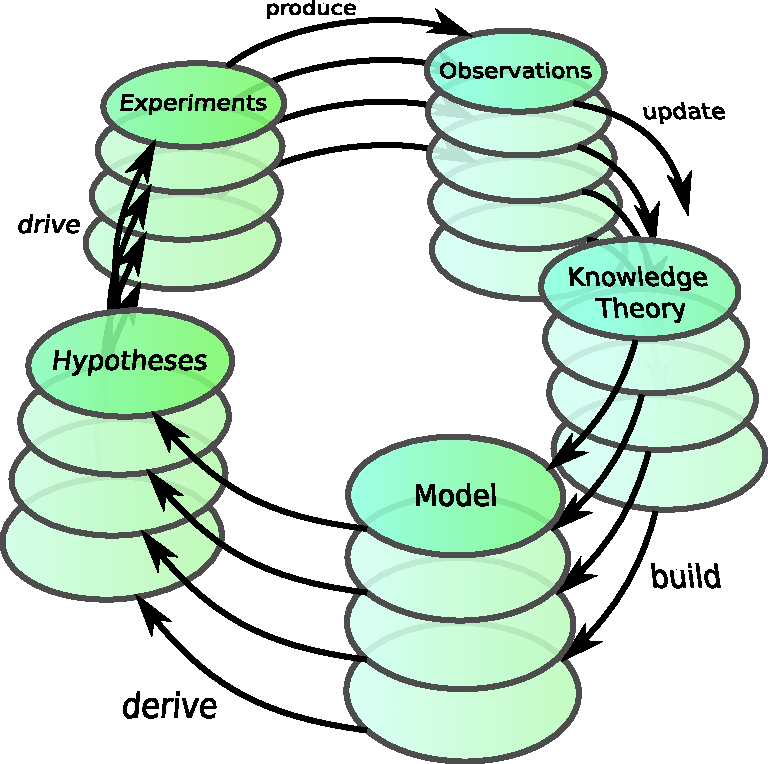
\includegraphics[width=0.35\textwidth]{images/empirical_spiral4}
%  \caption{The empirical spiral: applying the empirical cycle in successive
% rounds leads to a gradual build-up of knowledge.}\label{fig:empirical-spiral}
% \end{figure}






\begin{figure*}[htbp]
\begin{center}
%   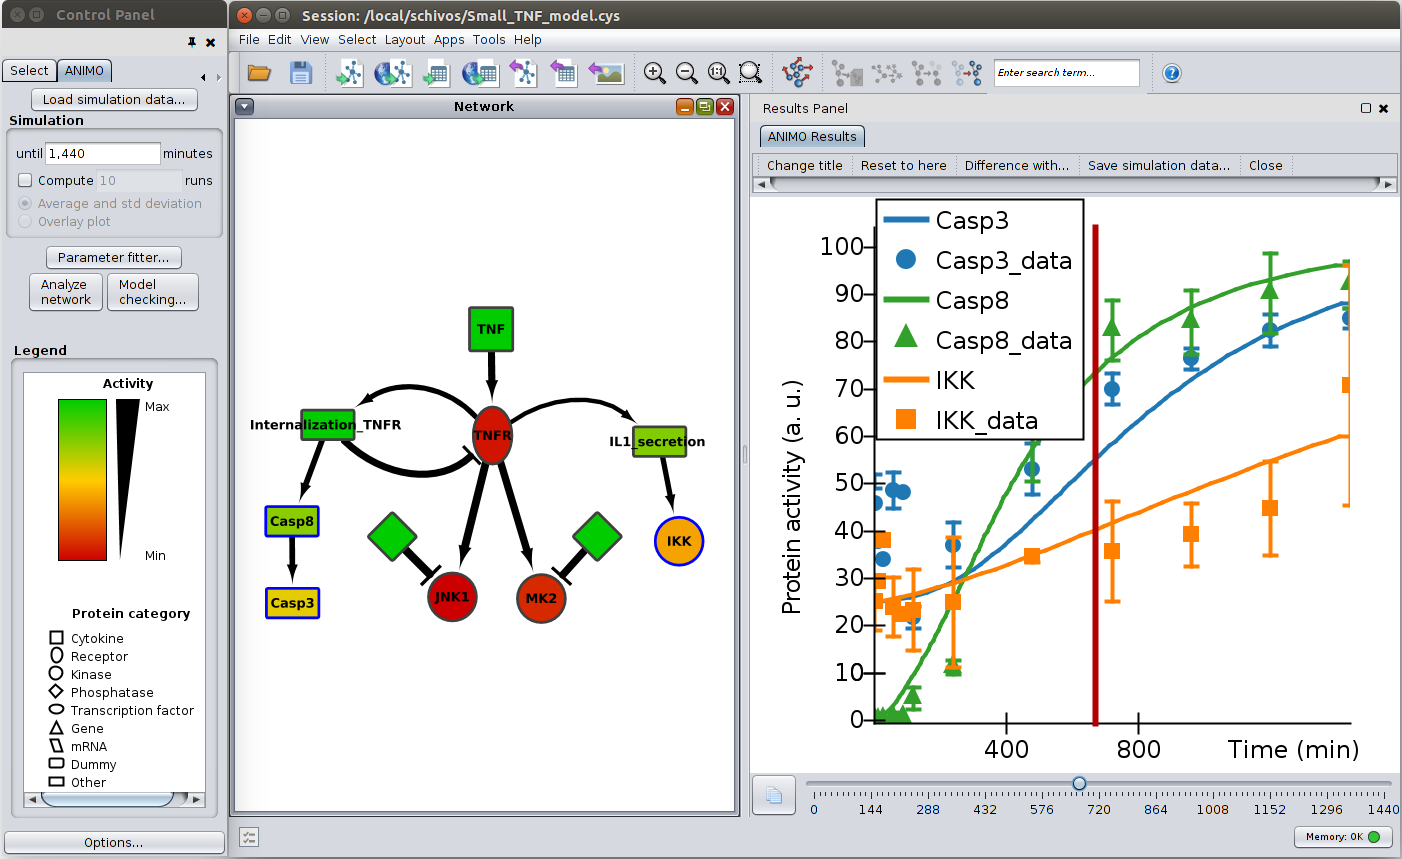
\includegraphics[width=.85\textwidth]{Figures/1}
\end{center}
\caption{\csentence{The Cytoscape user interface running the ANIMO plug-in.}
The \emph{Network} panel in the centre contains the nodes-edges
model of the example TNF$\alpha$ pathway (see Methods Section), with
colours indicating node activity levels and shapes representing different protein categories (see the \emph{Legend} on the left).
The \emph{Results Panel} on the right contains a graph plotting activity levels of selected nodes
during the first 24 hours of simulation of the model. The slider under the graph
allows the user to select the time instant (marked as a vertical red line in the graph) on which
the colours nodes in the \emph{Network} are based.
The series with the {\sf \_data} suffix is experimental
data from~\cite{pathway-compendium}, considering a treatment with 100~ng/ml TNF$\alpha$.\\
All acronyms used in this paper
and their corresponding UniProt IDs are listed in Suppl. Sect.~A. %\ref{suppl-sec:names}.
\label{fig:cytoscape}}
\end{figure*}

\begin{figure*}[htbp]
 \begin{center}
%   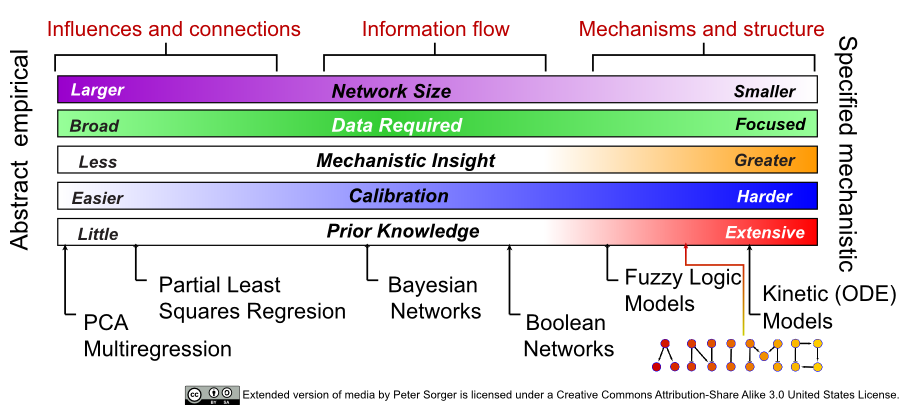
\includegraphics[width=0.9\textwidth]{Figures/2}
 \end{center}
\caption{\csentence{The spectrum of modelling methods, with the addition of ANIMO.}
The precision of ANIMO models is halfway between fuzzy logic and ODE. Compared to other
modelling tools, ANIMO
allows for an easier modelling experience thanks to a user-friendly interface based on
the widely used network modelling software Cytoscape.\label{fig:animo-spectrum}}
\end{figure*}

\begin{figure*}[!htpb]
\begin{center}
%   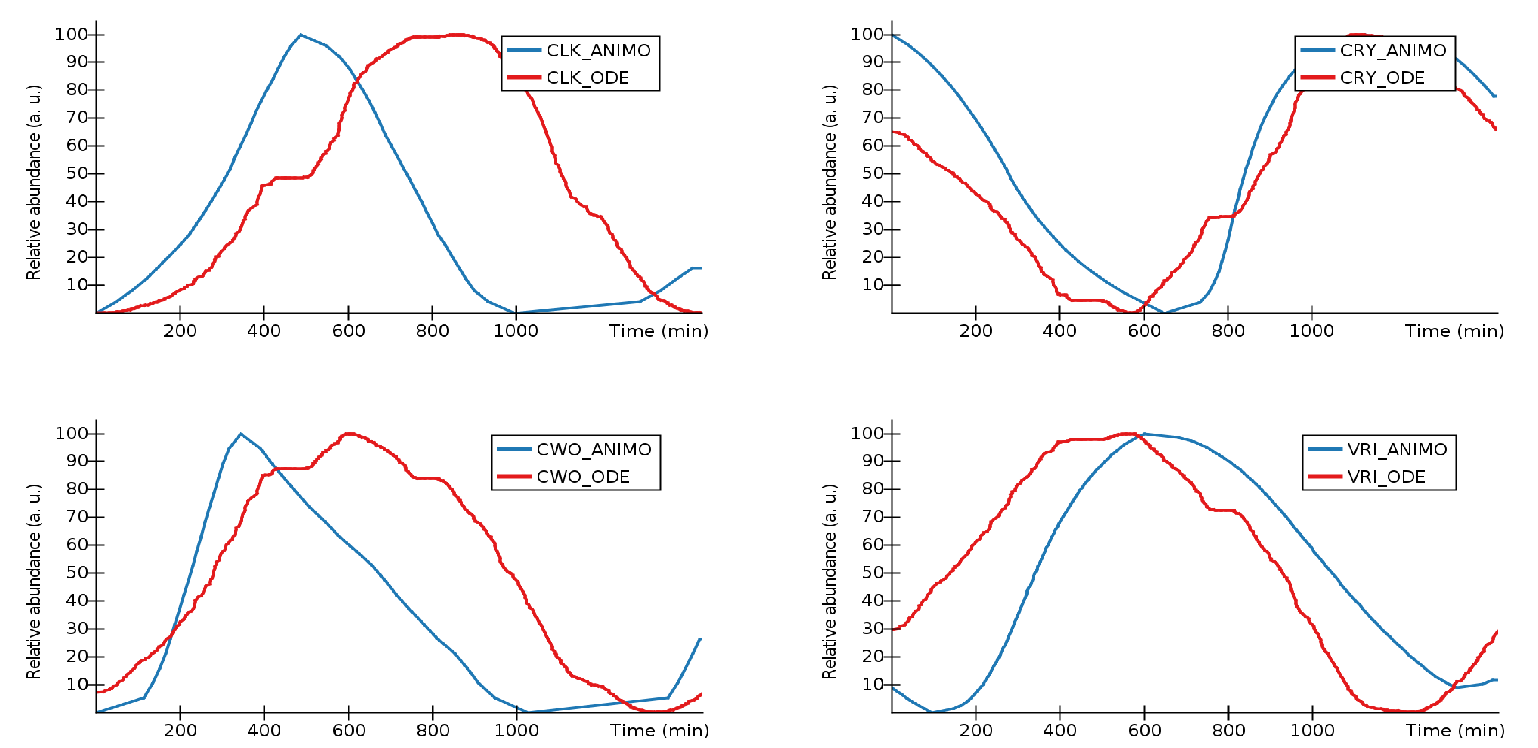
\includegraphics[width=0.9\textwidth]{Figures/3.pdf}
\end{center}
\caption{\label{fig:grafici-drosophila-smaller}\csentence{Comparing the result of the ANIMO model of \emph{Drosophila Melanogaster} circadian clock
with the model of~\cite{drosophila-ode-model}.} 24 hours simulations of the two models were compared
against each other, synchronizing their start point as much as possible. The blue line is the ANIMO model
({\sf \_{}ANIMO} series), while the red line represents the data computed from the original ODE model
({\sf \_{}ODE} series). The vaules of all series were rescaled on a [0, 100] interval to facilitate comparison.}
\end{figure*}


\begin{figure*}[!htpb]
\centering
%   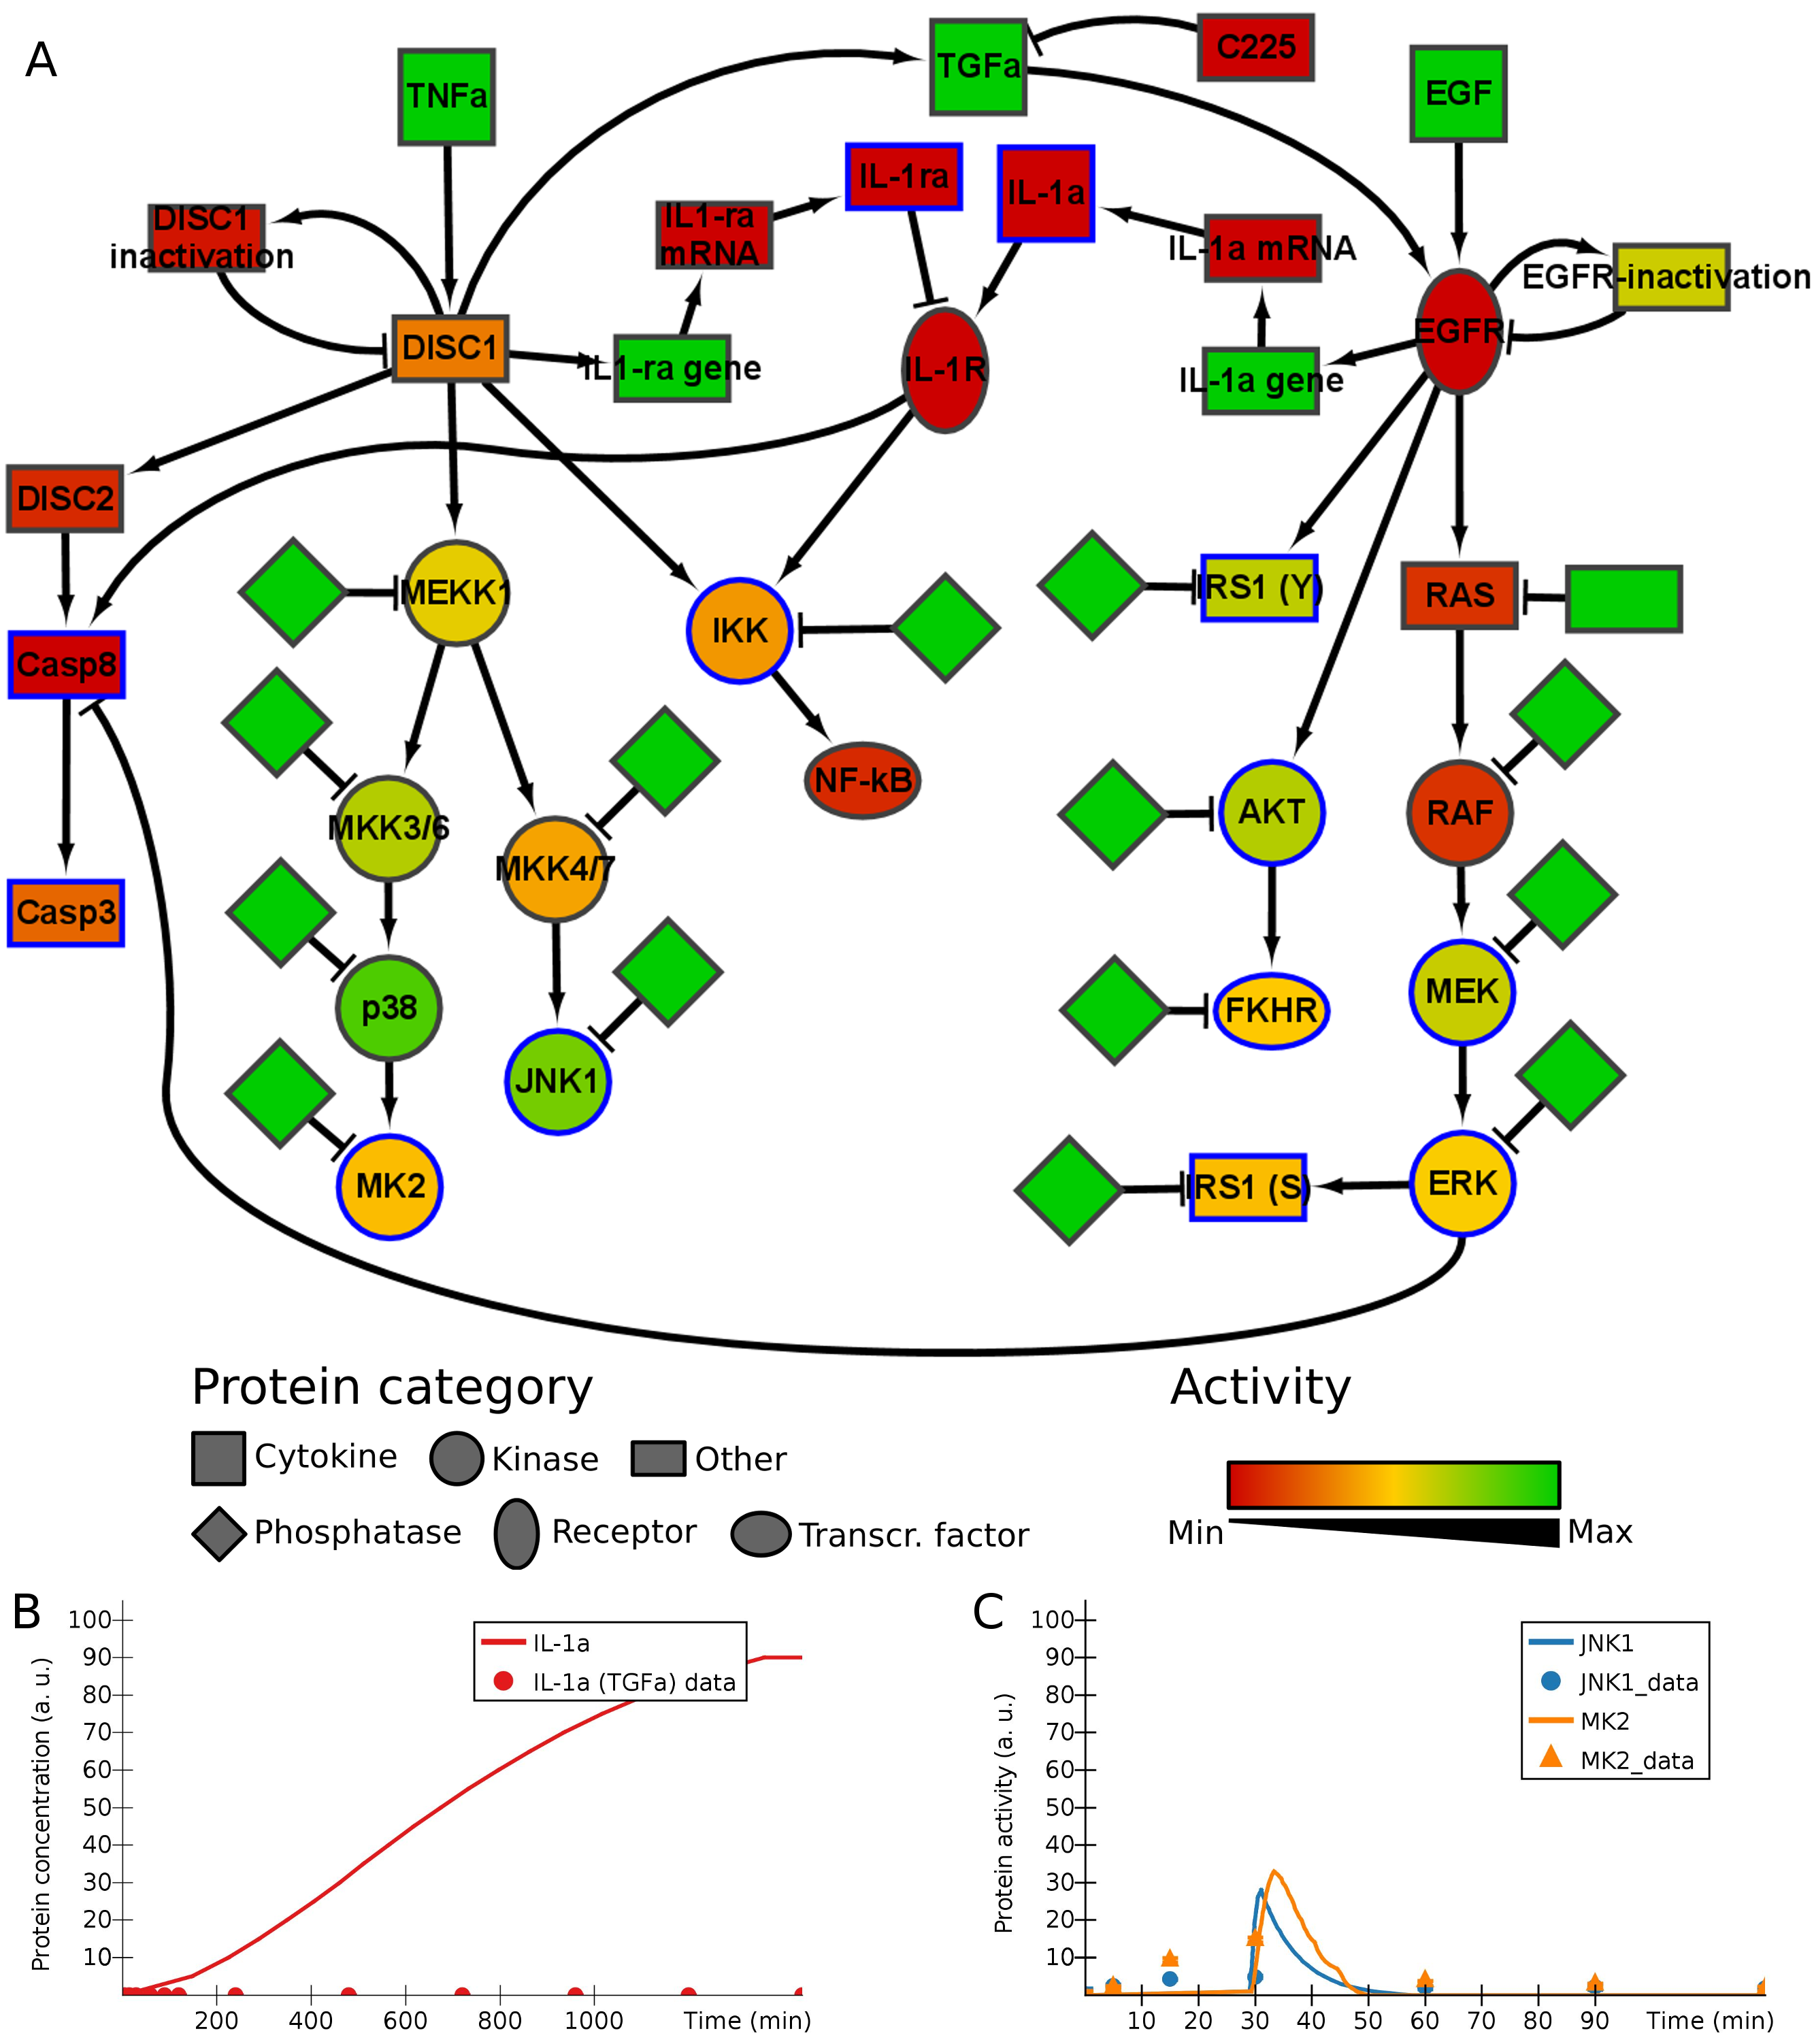
\includegraphics[width=0.9\textwidth]{Figures/4}
\caption{\csentence{Signalling network downstream of TNF$\alpha$ and EGF in human colon carcinoma cells.}
{\bf(A)}
The model for the merged TNF$\alpha$ and EGF pathways. Node colours represent the
activity level of the corresponding modelled reactants at time $t = 15$ minutes after
a stimulation of 100 ng/ml TNF$\alpha$ + 100 ng/ml EGF.
{\bf(B)}
Modelled production of IL-1$\alpha$ after stimulation with 100 ng/ml TGF$\alpha$ (24 hours).
{\bf(C)}
Modelled activation of JNK1 and MK2 after stimulation with 5 ng/ml TNF$\alpha$ + 10 $\mu$g/ml C225 (2 hours).
\\
The {\sf \_{}data} suffix identifies experimental data; all other series are computed by ANIMO.}\label{fig:large-model-all}
\end{figure*}

\begin{figure*}[!htpb]
\begin{center}
%   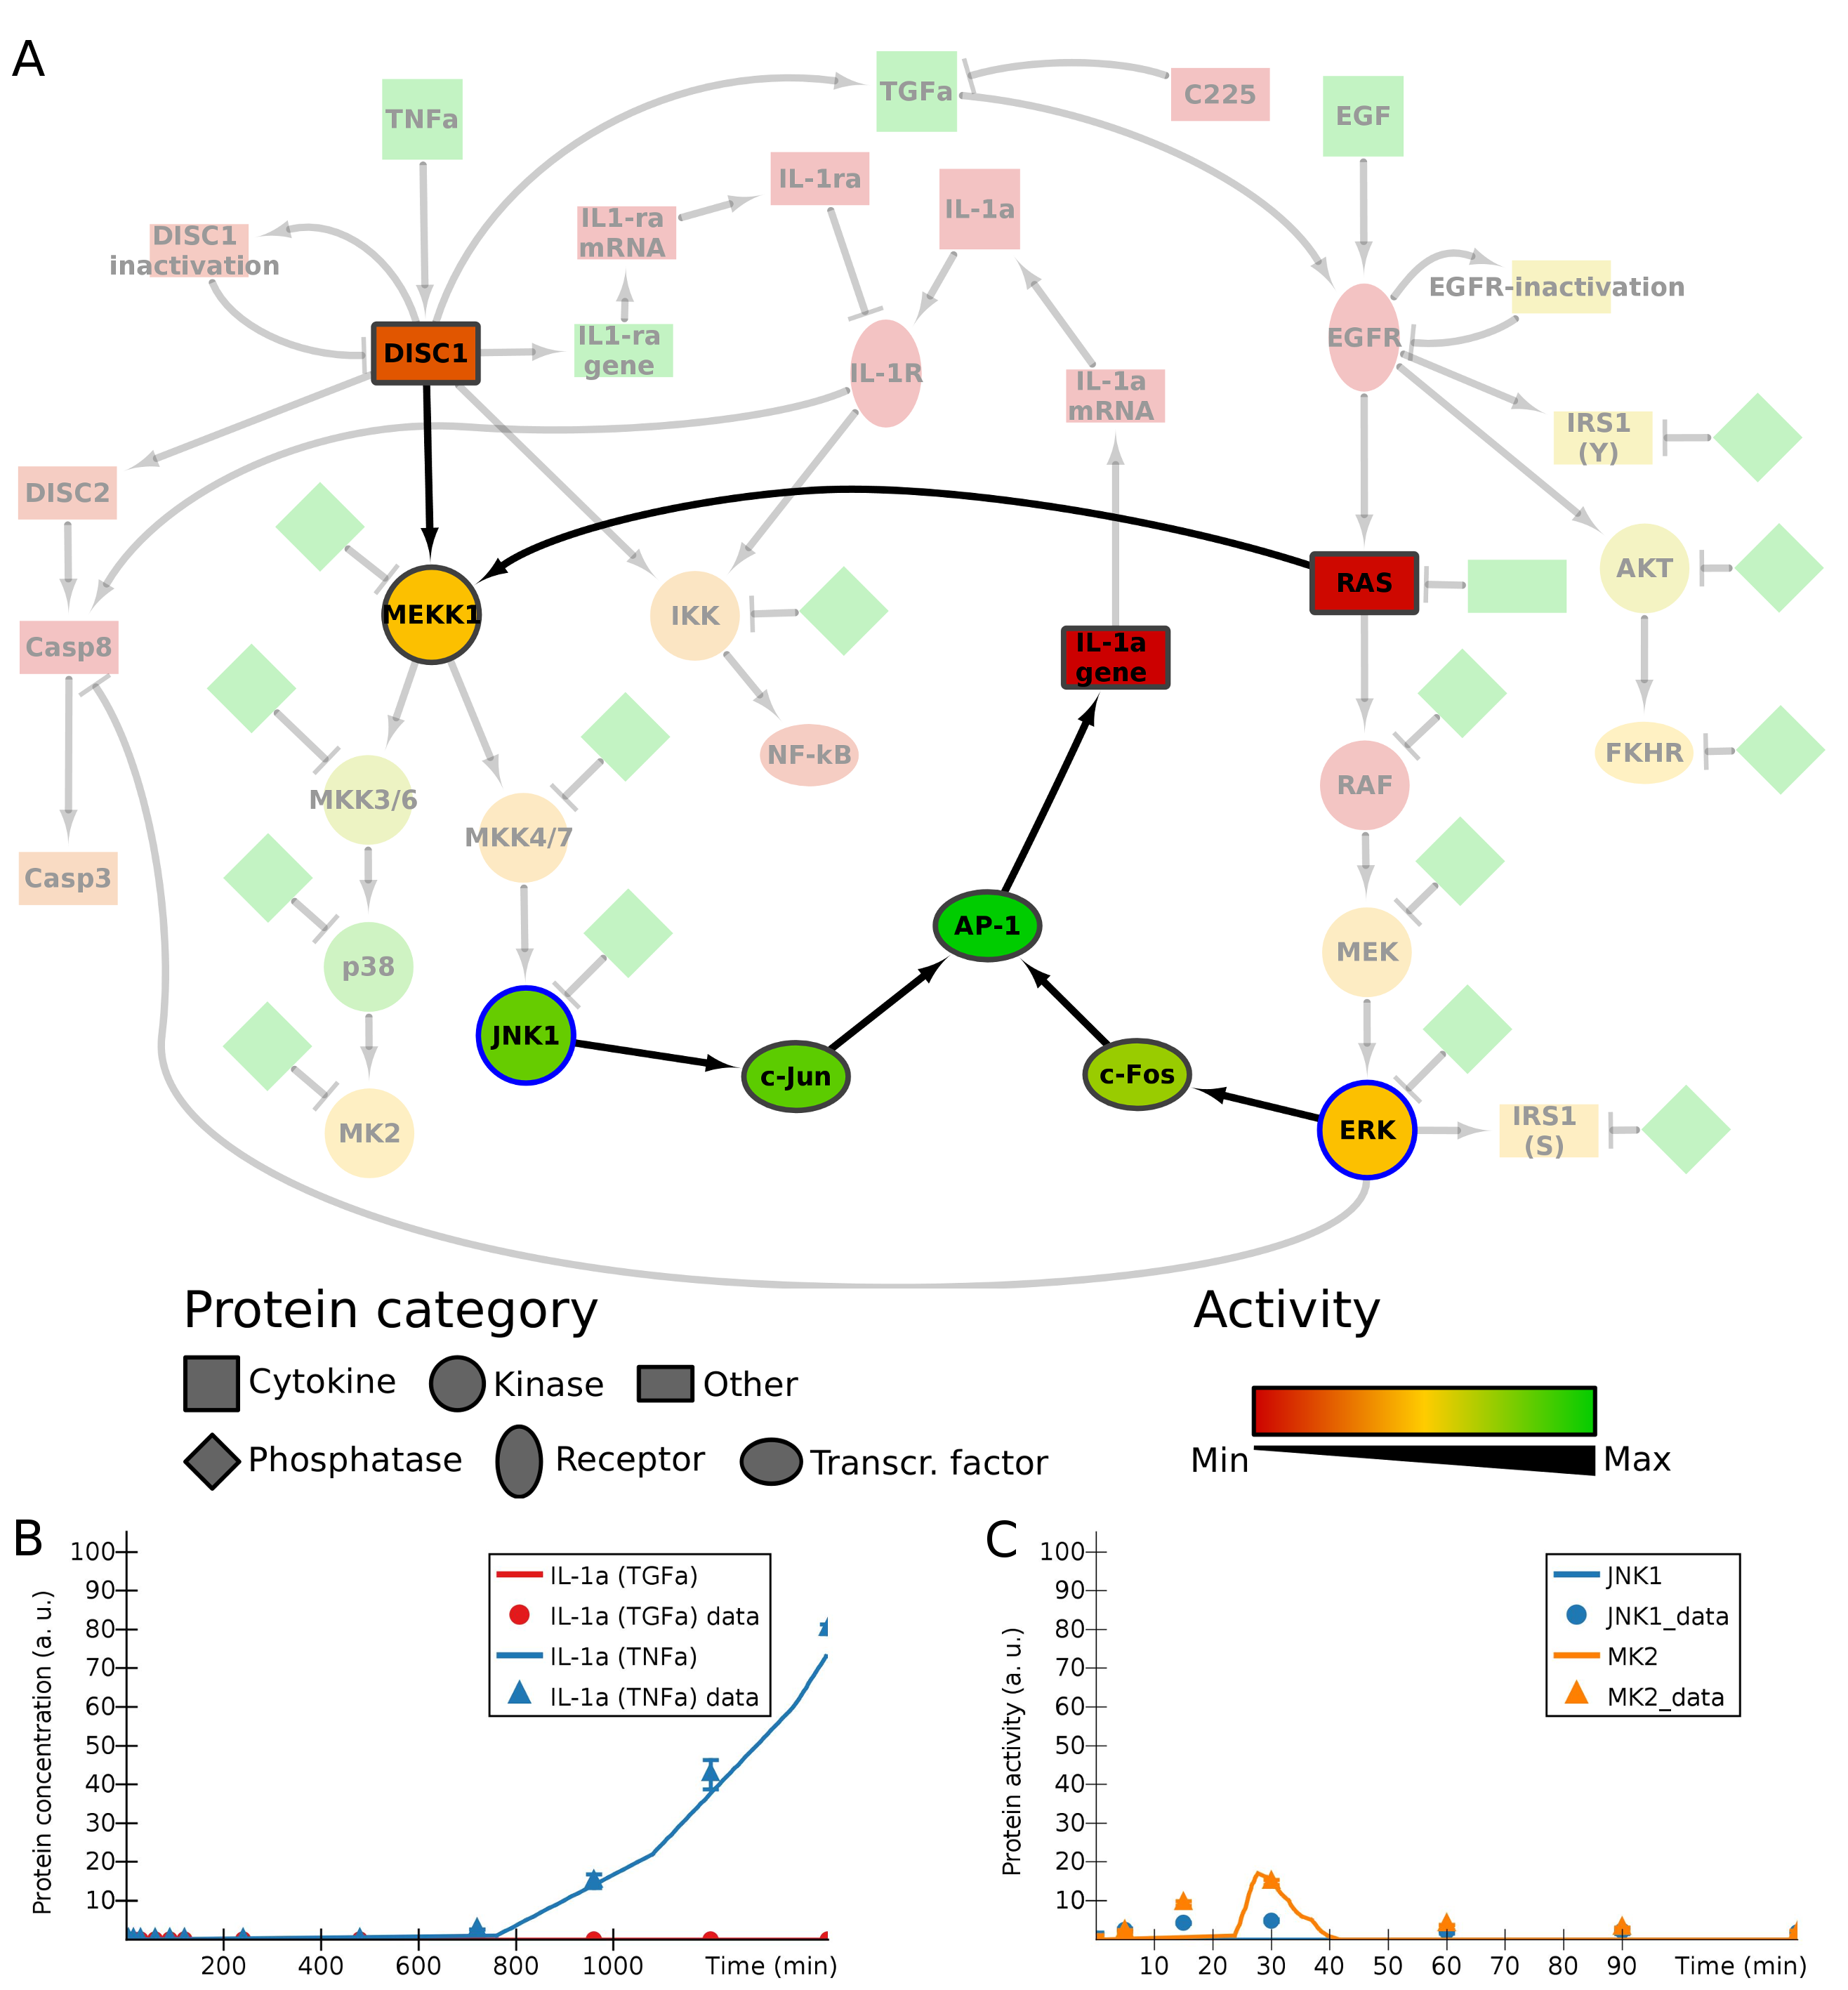
\includegraphics[width=0.9\textwidth]{Figures/5}
\end{center}
\caption{\csentence{Signalling network downstream of TNF$\alpha$ and EGF in human colon carcinoma cells: improved model.}
{\bf(A)}
The model for the merged TNF$\alpha$ and EGF pathways
after addition of the two hypotheses (highlighted).
Hypothesis~1 assumes IL-1$\alpha$ expression to depend on AP-1 activity, which in turn requires
both c-Jun en c-Fos to be activated by JNK1 and ERK, respectively. Hypothesis~2 assumes RAS as an activator
of MEKK1. Node colours represent the activity levels $15$ minutes
after stimulation of 100 ng/ml TNF$\alpha$ + 100 ng/ml EGF.
{\bf(B)}
After the addition of the first hypothesis (activation of IL-1$\alpha$ production depending both
on JNK1 and ERK): production of IL-1$\alpha$ after stimulation with 100 ng/ml TNF$\alpha$ (series {\sf IL-1a~(TNFa)})
compared with stimulation with 100 ng/ml TGF$\alpha$ (series {\sf IL-1a~(TGFa)}) (24 hours). The {\sf IL-1a (TGFa)} series is always 0.
{\bf(C)}
After the addition of the second hypothesis (activation of MEKK1 downstream of EGFR):
activation of JNK1 and MK2 after
stimulation with 5 ng/ml TNF$\alpha$ + 10 $\mu$g/ml C225 (2 hours). The {\sf JNK1} series is always 0.
Suppl. Sect.~D.4 %\ref{suppl:parameters-tnf-egf} 
explains how the dosage of 5 ng/ml TNF$\alpha$ was represented in the model.\\
The {\sf \_{}data} suffix identifies experimental data; all other series are computed by ANIMO.}\label{fig:large-model-complete}
\end{figure*}


\begin{figure*}[!h]
\begin{center}
%   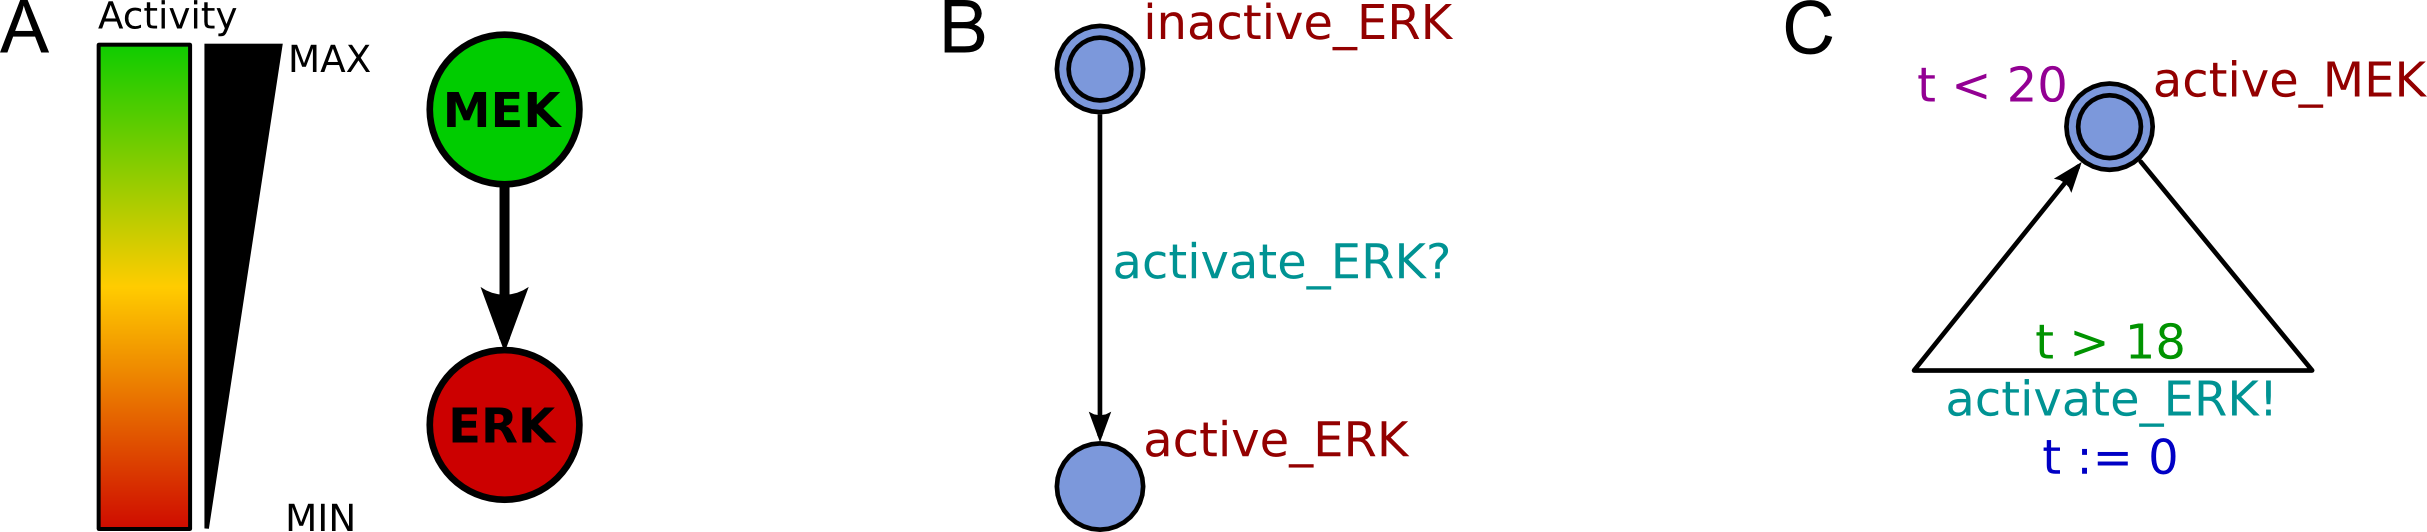
\includegraphics[width=0.8\textwidth]{Figures/6}
\end{center}
\caption{\csentence{Abstraction of a biochemical reaction to a \tas\ model.}
{\bf(A)}
Classical depiction of a well-studied intracellular signal transduction reaction: protein
MAPK-ERK kinase (MEK) activates downstream protein extracellular-regulated kinase (ERK).
{\bf(B)}
A \ta\ model of ERK, consisting of two locations (circles), {\sf inactive\_ERK} and {\sf active\_ERK},
and one transition (arrow) between the locations. This transition will take place when it is possible to synchronize with
the corresponding action {\sf activate\_ERK!} in the MEK automaton.
{\bf(C)}
A \ta\ model of active MEK, consisting of one location and one
transition. ${\sf t} < 20$ is called an invariant on the location, allowing residence in this location as long as 
clock time {\sf t} is smaller than $20$ units. ${\sf t} > 18$ is called a guard on the transition, allowing the
transition to take place when clock {\sf t} is greater than $18$ units. Together, the invariant and guard in this
example ensure that the transition must take place in the (continuous) time interval $18 < {\sf t} < 20$. When the
transition takes place, the action {\sf activate\_Erk!} is performed (thus allowing the ERK automaton to reach the {\sf
active\_ERK} location) and the local clock coupled to this automaton is reset, ${\sf t} := 0$.\label{fig:abstraction-mek-erk}}
\end{figure*}

\begin{figure*}[!htbp]
\centering
%   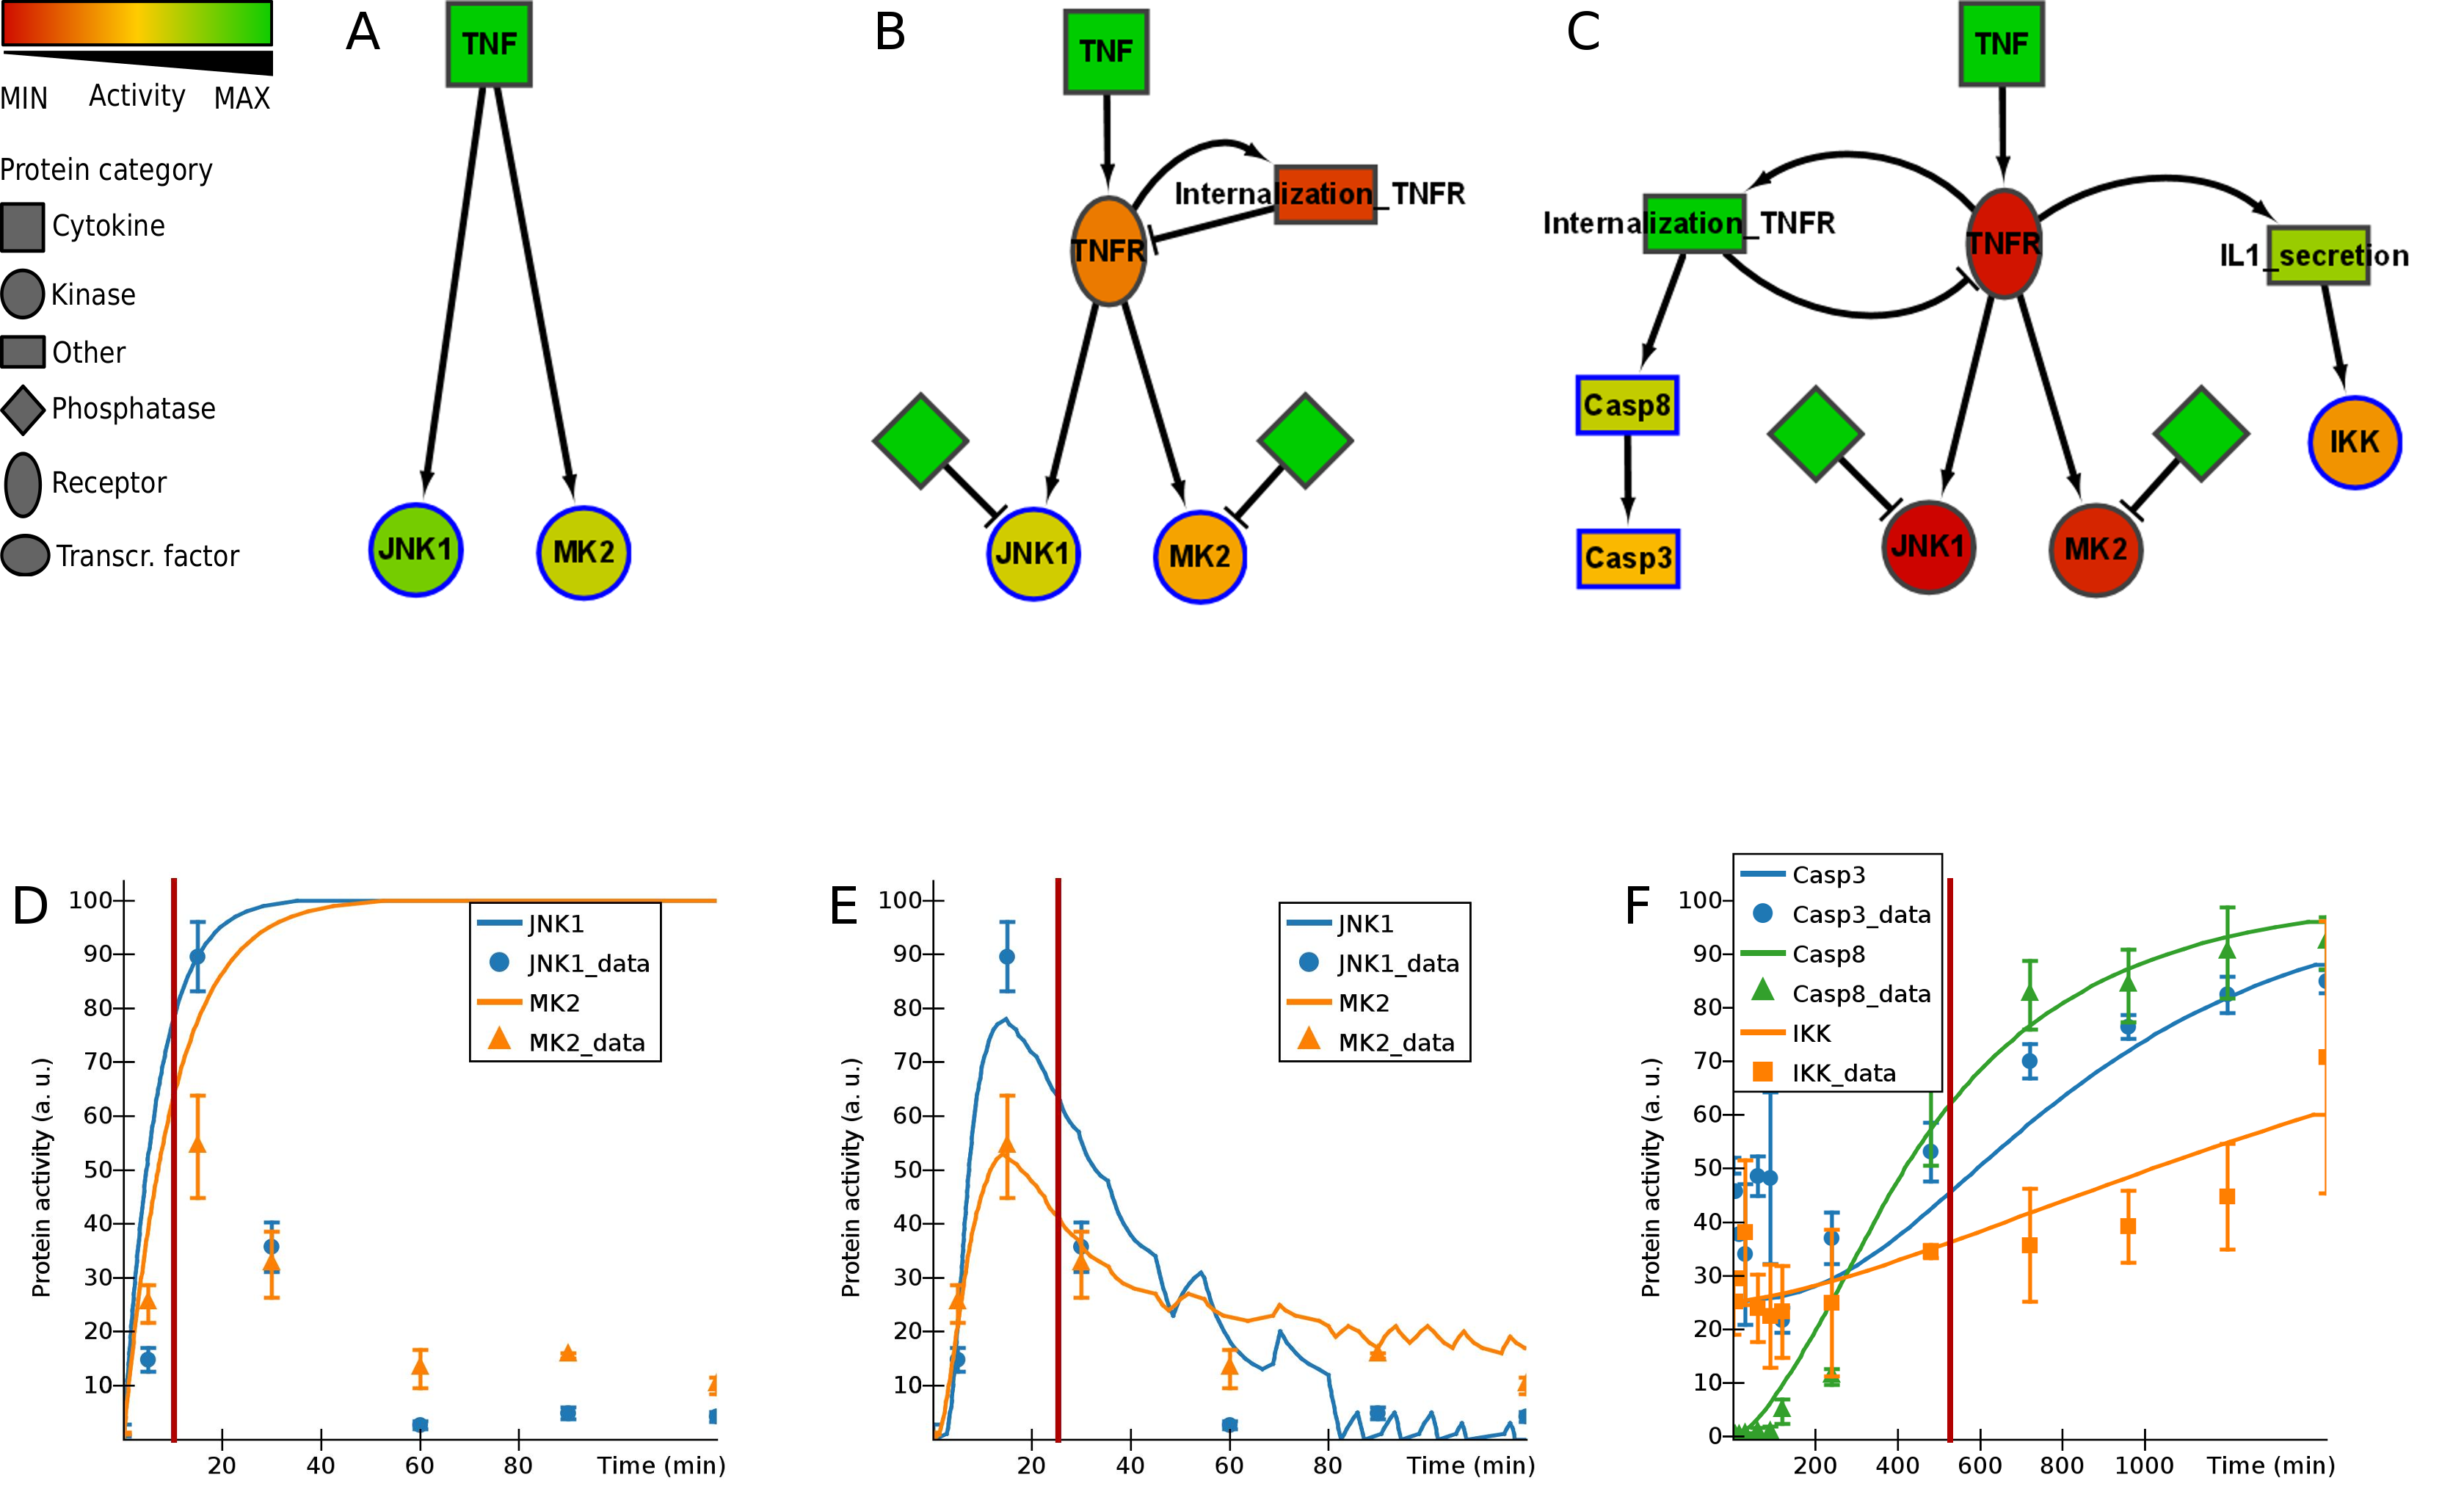
\includegraphics[width=0.9\textwidth]{Figures/7}
  \caption{
\csentence{Construction of an ANIMO model of signal transduction
events in human colon carcinoma cells upon stimulation with 100 ng/ml TNF$\alpha$.}
Graphs below show the dynamic behaviour of the corresponding models above, comparing it to the measured
activity values from~\cite{pathway-compendium} (error bars represent the standard deviation).
On the vertical axis, ``100'' represents the maximum protein activity in the complete experiment.
A red vertical line in each graph highlights an arbitrary time point in the time course:
nodes in the corresponding model are coloured according to their activity at that time point.
{\bf(A,~D)}
Basic model showing direct activation of JNK1 and MK2 by TNF$\alpha$.
No peak dynamics are observed because no inactivating processes are present.
{\bf(B,~E)}
The model after addition of inactivating phosphatases and a negative feedback loop that down-regulates TNFR.
Note that adding TNFR internalization or phosphatases alone would not be enough to reproduce activity peaks.
{\bf(C,~F)}
The model after addition of IKK, IL1-secretion (abstracting
the autocrine IL-1 signalling described in~\cite{pathway-autocrine}), Casp8 and Casp3, showing the late response to TNF$\alpha$ signalling.
As the data set did not contain values for cleaved caspase-3, but only for its non-cleaved precursor pro-caspase-3,
we computed the {\sf Casp3\_{}data} series as $100\% - [\mbox{\sf pro-Casp3}]$.\label{fig:small-model}}
\end{figure*}







%%%%%%%%%%%%%%%%%%%%%%%%%%%%%%%%%%%
%%                               %%
%% Tables                        %%
%%                               %%
%%%%%%%%%%%%%%%%%%%%%%%%%%%%%%%%%%%

%% Use of \listoftables is discouraged.
%%
\clearpage
\section*{Tables}
% % \begin{table}[h!]
% % \caption{Sample table title. This is where the description of the table should go.}
% %       \begin{tabular}{cccc}
% %         \hline
% %            & B1  &B2   & B3\\ \hline
% %         A1 & 0.1 & 0.2 & 0.3\\
% %         A2 & ... & ..  & .\\
% %         A3 & ..  & .   & .\\ \hline
% %       \end{tabular}
% % \end{table}


\newcolumntype{x}[1]{%
>{\centering\hspace{0pt}}p{#1}}%
% \savenotes
\begin{table*}[!hbt]
\begin{minipage}{\textwidth}
\begin{center}
{\scriptsize \begin{tabular}{p{3cm}p{1.2cm}p{1.1cm}p{1.2cm}p{1cm}p{1cm}p{1cm}}
\hline \ \\
{\bfseries Tool} & {\bfseries Formalism} & {\bfseries Domain-specific interface} & {\bfseries Visual modeling} & {\bfseries Qualitative parameters} & {\bfseries Tight coupling with topology} & {\bfseries User-chosen granularity}  \\[5mm]
\hline \ \\
ANIMO~\cite{animo-bibe} & Timed \ \ \ Automata & Yes & Yes & Yes & Yes & Yes
      \\[5mm]
Bio-PEPA Workbench~\cite{biopepa-interface} & Bio-PEPA & No & No & No & No & Yes
      \\[5mm]
Cell Illustrator~\cite{cell-illustrator} & Petri Nets & Yes & Yes & No & Yes & No
     \\[5mm]
COPASI~\cite{copasi} & ODE, stochastic models & No & No & No & No & No
      \\[5mm]
COSBI LAB~$^1$
 & BlenX & Yes & Yes & No & Yes & No
      \\[5mm]
GINsim~\cite{ginsim} & Boolean Networks & No & Yes & Yes & Yes & Yes~$^2$
      \\[5mm]
GNA~\cite{gna}    & PLDE & No & Yes & Yes & Yes & Yes~$^2$
      \\[5mm]
Rhapsody~$^3$
 & Statecharts & No & Yes & Yes & No~$^4$ & No
      \\[5mm]
\hline \ \\
\end{tabular}}
\end{center}
\end{minipage}
\caption{Comparison between ANIMO and some existing approaches to modelling biological systems.
A ``Yes'' under a column indicates that the modelling tool (mostly) fulfils the parameter, ``No'' indicates very limited or no fulfilment.\\
$^1$ {COSBILab} web page \protect\url{http://www.cosbi.eu/index.php/research/cosbi-lab}\\
$^2$ The user can choose the number of levels for each reactant, allowing to define
multi-level models based on Boolean reaction dynamics.\\
$^3$ {IBM Rational Rhapsody} web page \protect\url{http://www-01.ibm.com/software/rational/products/rhapsody/designer}\\
$^4$ Statecharts represent more closely the so-called \protect\emph{transition system} of the model as opposed to the components and interactions occurring among them.
\label{tab:tool-comparison}}
\end{table*}




%%%%%%%%%%%%%%%%%%%%%%%%%%%%%%%%%%%
%%                               %%
%% Additional Files              %%
%%                               %%
%%%%%%%%%%%%%%%%%%%%%%%%%%%%%%%%%%%

\clearpage

\section*{Additional Files}
  \subsection*{Additional file 1 --- ANIMO models and data for the case studies}
      The provided .zip file contains the Cytoscape .cys network files which can be analysed
      with ANIMO. In addition, the reference values in .csv format are provided, to compare
      ANIMO's results with the previously existing models. In order to grant a fair comparison,
      note that ANIMO's results need to be rescaled the same way as the ODE results
      (i.e. normalize each series w.r.t. to its minimum and maximum) before the comparison.


\end{backmatter}


\end{document}
